\begin{figure*}[t!]
\centering
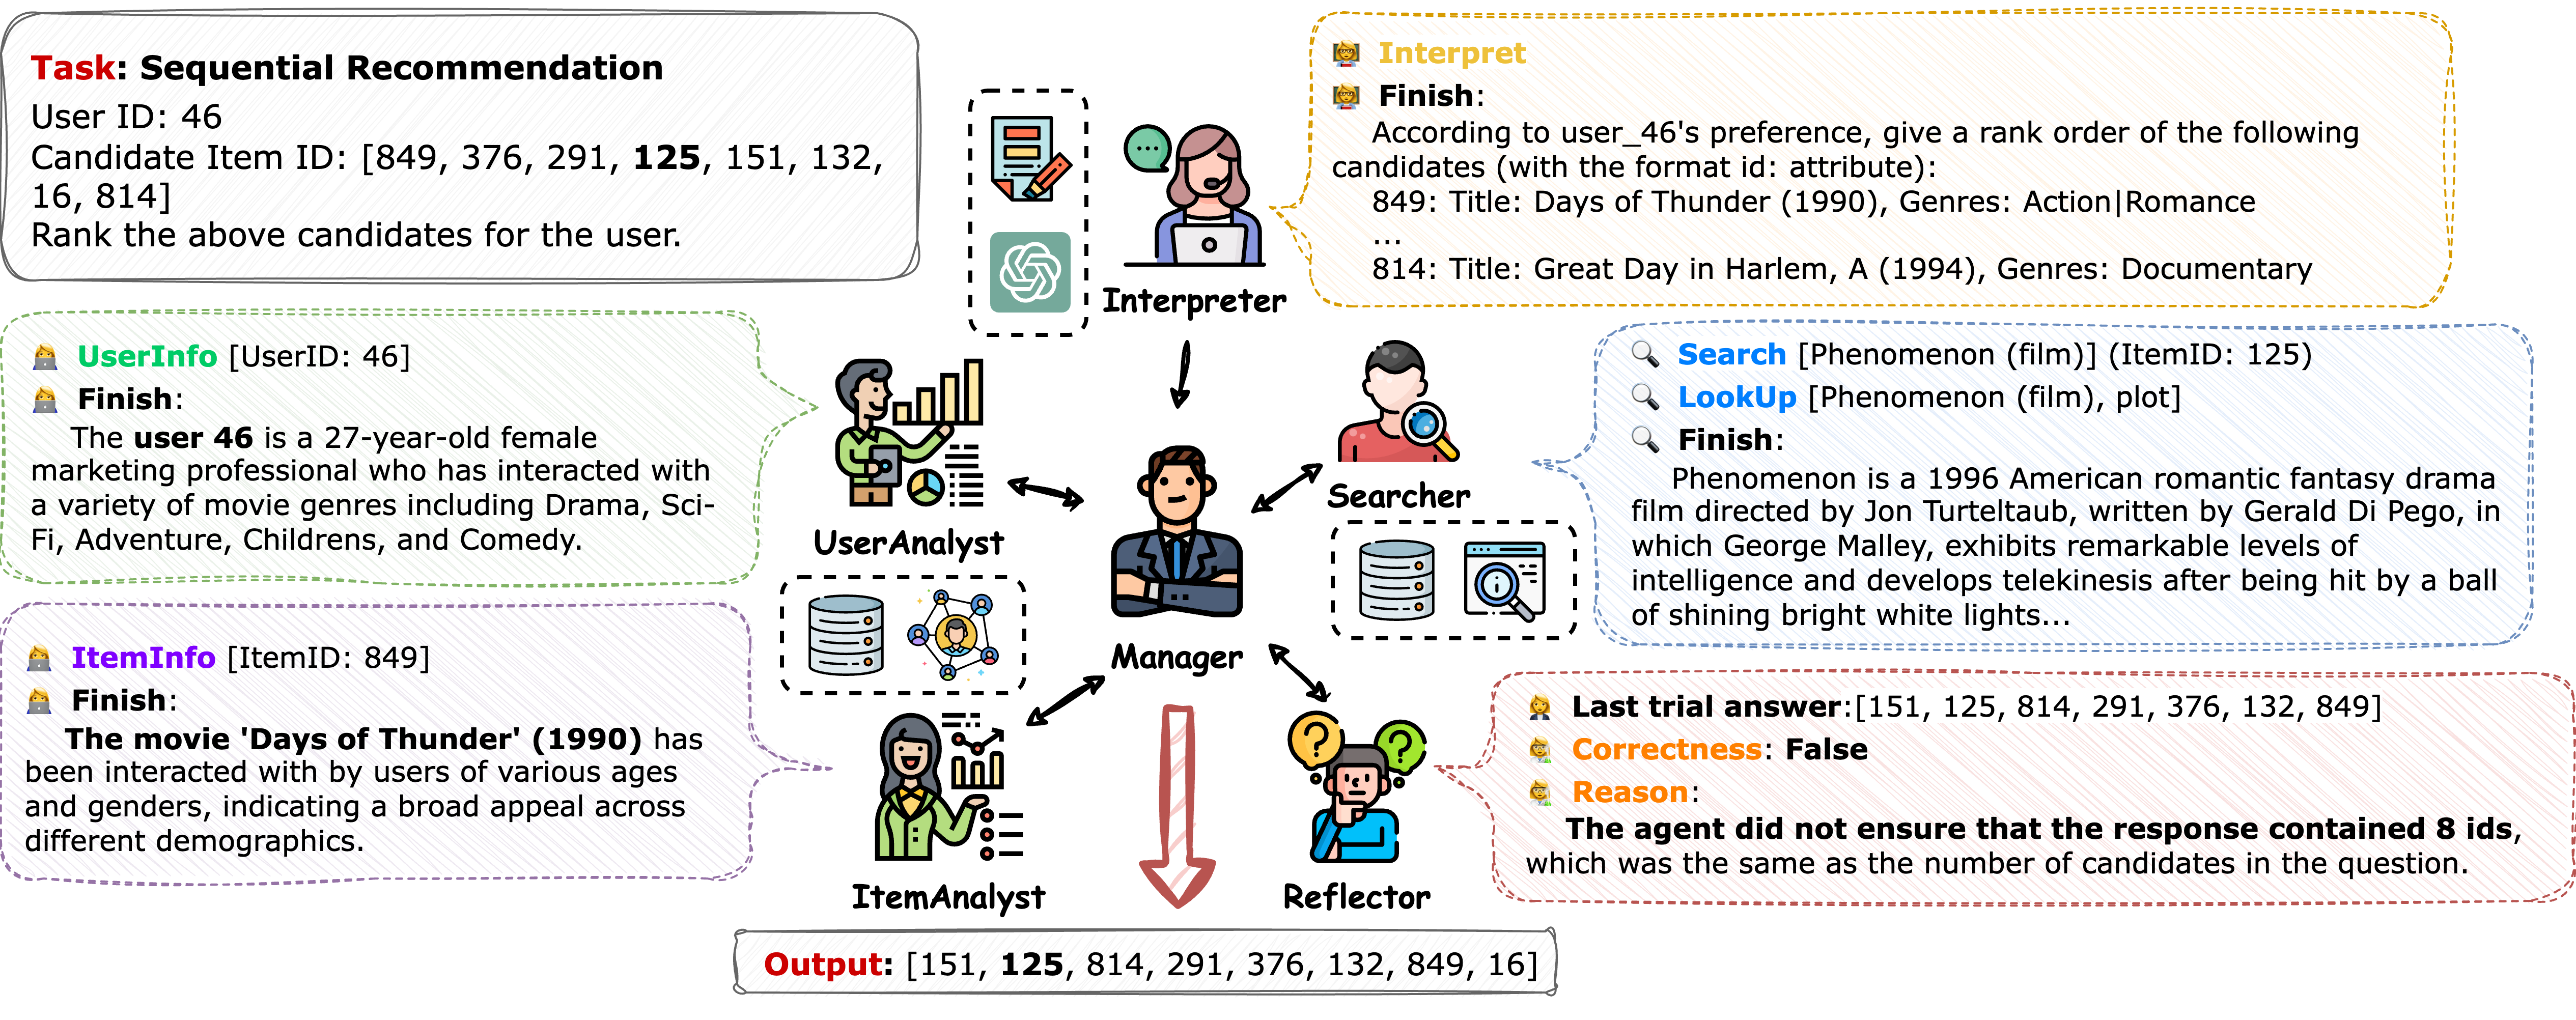
\includegraphics[trim={0 0 0 0}, clip, width=0.9\textwidth]{Figures/MAC-workflow.png}
\caption{The Framework of MACRec. We take a sequential recommendation task as an example to show how these agents work collaboratively.}
\Description[The framework of MACRec.]{The framework of MACRec.}
\label{fig:framework}
\end{figure*}

\section{The MACRec Framework}

\subsection{Framework Overview}

Figure~\ref{fig:framework} illustrates our proposed multi-agent collaboration recommendation framework.
% Framework Overview
% 以图中的sequential recommendation任务为例
A sequential recommendation task is given as an example.

% The \textsl{Manager} is always placed at the center during the running process.
% All other types of agents serve as the assistant role for the \textsl{Manager}.
% 所有的agents以Manager为中心，共同协作完成任务。
% All agents work together to complete the task with the \textsl{Manager} at the center.
% 每个agent有各自的特长，对于给定的任务在完成后会将结果反馈给Manager。
% Each agent has its expertise and will provide feedback on the given sub-task from \textsl{Manager}.
% 一部分Agents支持对工具的调用，如Searcher、Analyst和Task Interpreter。
% In the example provided in Figure~\ref{fig:framework}, 
As shown in the example in Figure~\ref{fig:framework}, 
the \textsl{Task Interpreter} first translates the task in a better way to understand.
Then, as the central component of the entire system, the \textsl{Manager} starts calling other agents to obtain detailed analyses of the user and items.
These agents, including the \textsl{Searcher} and the \textsl{User/Item Analyst}, support the call of some tools, 
% Additionally, some agents support the call of tools, 
% such as the \textsl{Searcher} and the \textsl{User/Item Analyst}.
e.g., the \textsl{Searcher} has access to the search engine and the \textsl{User/Item Analyst} can access detailed information about users and items.
% Manager 1st
After receiving responses from the \textsl{Searcher} and \textsl{Analyst}, the \textsl{Manager} will attempt to provide an answer, i.e., give a ranking order of the candidate sets.
% 解释reflector（每个agent都出现一次）
The \textsl{Reflector} will be responsible for analyzing and reflecting on the \textsl{Manager}'s answer in the last trial and giving suggestions, e.g., modifying the answer format to follow the task requirements.
Eventually, the Manager will reattempt to solve the task based on the reflections and provide a more reasonable answer, e.g., adding the missed item ID.

% 具体每个agent的特点与功能将在下文详细介绍。
The following sections will detail each agent's specific characteristics and functions.\footnote{Code is available at \href{https://github.com/wzf2000/MACRec}{https://github.com/wzf2000/MACRec}.}

% % 我们为不同的推荐场景设计了五类具有各异特长的agents。
% We designed five types of agents with different specialties for different recommendation scenarios.

% \begin{figure}[t!]
% \centering
% 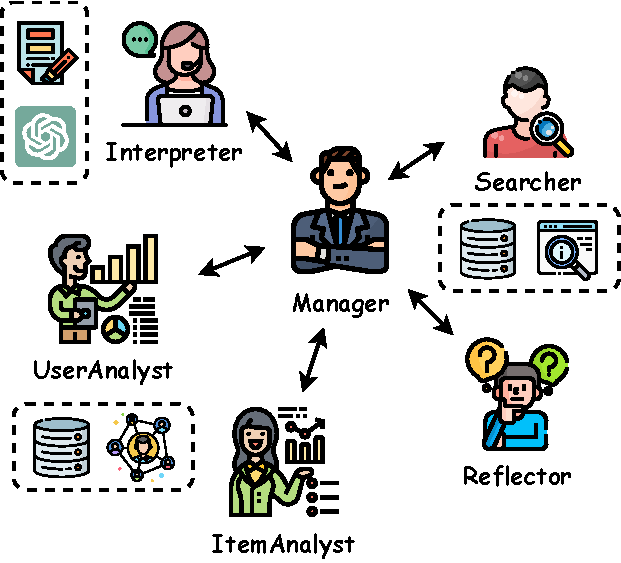
\includegraphics[trim={0 0 0 0}, clip, width=0.3\textwidth]{Figures/MACRec-Framework.pdf}
% \caption{The framework of MACRec.}
% \label{fig:framework}
% \end{figure}

% 改一下 summarized， id 46  id 151(Days of Thunder)  (phenomenon) 加上最终输出 加上标号 1 2 3 4 5  题目里写清楚 是一轮的 让底部对齐

\subsection{Agent Roles}

\subsubsection{\textbf{Manager}}
For the given task, the \textsl{Manager} would assign sub-tasks to other agents and complete the main execution process. It oversees the collaboration among all other agents. %, acting like a manager.

% Manager总是交替的执行思考、行动和观察三个步骤。
The \textsl{Manager} always performs the three steps of \textsl{Thought}, \textsl{Action}, and \textsl{Observation} alternately.
% 在思考阶段，Manager会推理当前任务的状态（如分析是否充足，是否需要额外信息等）。
In the \textsl{Thought} phase, the \textsl{Manager} reasons about the current situation of the task (e.g., whether the analysis is sufficient, whether additional information is needed, etc.).
% 而在行动阶段，Manager可选择给出答案结束任务，或是寻求其他agents的帮助。
During the \textsl{Action} phase, the \textsl{Manager} can choose to give an answer to end the task or seek help from other agents (under a particular interface format).
% 其他agents给出的回复将在Manager的observation阶段中给出。
Responses given by other agents will be given in the \textsl{Observation} phase of the \textsl{Manager}.

\subsubsection{\textbf{Reflector}}

The \textsl{Reflector} is responsible for judging the correctness of the answer given by the Manager. A further reflection will be given if the \textsl{Reflector} determines the answer is correct.

% 当Manager即将对同一个任务输入执行第二轮或更多的运行时，Reflector将会介入。
The \textsl{Reflector} will step in when the \textsl{Manager} is about to perform the second or more runs on the same task input.
% 如果Reflector判定Manager给出的答案没有可改进之处，Manager将会不再执行本轮运行，而是延续上一轮的答案。
If the \textsl{Reflector} judges that the answer given by the \textsl{Manager} has no room for improvement, the \textsl{Manager} will no longer perform the current run. % and continue the answer from the previous round.
% 否则，Reflector会进一步总结Manager的可改进之处，如未考虑到用户历史交互序列中的少数高分商品/电影等。
Otherwise, the \textsl{Reflector} will further summarize where the \textsl{Manager} can be improved, e.g., not considering the few highly rated items/movies in the user's historical interactions.

\subsubsection{\textbf{User/Item Analyst}}

\textsl{User/Item Analyst} specializes in examining and understanding the characteristics and preferences of users, as well as the attributes of items.

% Analyst在运行时将会获得所要分析的交互id对，即用户id与物品id。
% The \textsl{Analyst} will get the interaction ID pairs to be analyzed at runtime, i.e. the user ID and item ID.
% Analyst将会获得两类工具的调用权限以辅助分析。
The \textsl{Analyst} will be given access to two tools to assist in the analysis, including info database and interaction retriever.
% 可以通过Info database获得每个用户的用户画像和每个物品的属性信息。
The \textsl{Analyst} can get the user profile of each user and the attributes of each item through the info database.
% 通过Interaction retriever，Analyst可以获得在当前时间之前的用户/物品交互历史。
Through the interaction retriever, the \textsl{Analyst} can get the user/item interaction history before the current time.
% 通过这两种工具的结合，Analyst可以对用户和物品有深入的分析，从而给予Manager准确的建议。
With the combination of these two tools, the \textsl{Analyst} can have an in-depth analysis of the user or the item.

\subsubsection{\textbf{Searcher}}
% The \textsl{Searcher} is tasked with scanning the database or inventory to find items that match the criteria set by the recommendation system.

% Searcher负责将Manager给出的查询需求，配合搜索工具进行检索，最终总结出文本回复给Manager。
The \textsl{Searcher} is responsible for searching under the requirements given by the \textsl{Manager} with the search tool, and finally summarizing the text reply to the \textsl{Manager}.

% 以Wikipedia作为搜索工具为例。
Take Wikipedia as an example of a search tool.
% Searcher可以在通过给出query以获取在Wikipedia中相关度最高的几个词条。
The \textsl{Searcher} can give a search query to get the most relevant entry in Wikipedia.
% Searcher还可以进一步在具体的某个entry中检索存在相关字段的段落。
The \textsl{Searcher} can further retrieve passages in a specific entry where the given keywords exist.
% 通过检索得到结果与Manager给出查询需求的匹配程度，Searcher最终会总结出一段给Manager的文本回复。
Eventually, the \textsl{Searcher} is asked to summarize the paragraph to respond the the \textsl{Manager}'s query.
% Compared the retrieval results with the requirements given by the \textsl{Manager}, the \textsl{Searcher} will eventually summarize a paragraph to respond to the \textsl{Manager}.

\subsubsection{\textbf{Task Interpreter}}
The \textsl{Task Interpreter} translates the dialogs into executable recommendation tasks.

% Task Interpreter将得到用户与系统的对话历史。
The \textsl{Task Interpreter} will get the conversation history when starts running.
% 由于对话历史可能较为冗长，Task Interpreter只会得到历史的最后一部分。
Since conversation histories can be long, the \textsl{Task Interpreter} will only get the last part of the history.
% 同时，Task Interpreter还可以通过文本摘要工具以得到更精炼的历史概括。
The \textsl{Task Interpreter} also has access to call the text summarization tool to get a more concise overview of the history.
% 最终，Task Interpreter会给出一个具体的任务需求描述，用以指导Manager后续的运行。
Eventually, the \textsl{Task Interpreter} will give a specific description of the task requirements that will be used to guide the subsequent runs of the \textsl{Manager}.


% \subsection{Collaborative Recommendation}

% In our multi-agent collaboration system, the \textsl{Manager} is always placed at the center.
% All other types of agents serve as the assistant role for the \textsl{Manager}.

% Some agents are executed by the \textsl{Manager}'s request, such as the \textsl{Searcher} and the \textsl{User/Item Analyst}.
% For the \textsl{Searcher} and the \textsl{Analyst}, the \textsl{Manager} has the right to choose cooperation or not independently.
% For the \textsl{Reflector} and the \textsl{Task Interpreter}, we execute it according to the predefined rules and use its results as an optional reference for the \textsl{Manager}.
% Manager在不同的系统中拥有不同的Action选项。
% The \textsl{Manager} has different Action options on different systems.
% 同时，根据Agents选取的不同，其任务描述也会对应更改。
% Meanwhile, depending on the selected agents and the task type, the prompts for the \textsl{Manager} will be changed accordingly.

% % Using GPT-3.5 as default; required to give answers to recommendation questions (give a rating or give a ranking of the candidates)
% The actor agent is responsible for completing the main execution process of the task.
% % 包含了任务描述和基本要求的prompt作为actor的输入。
% % translate it into English:
% The prompt containing the task description and basic requirements is used as the input of the actor.
% % prompt
% % 其中任务描述可参见图~\ref{fig:framework}，一般包含了用户id，用户画像，用户历史交互，任务回答要求、候选集等信息。
% An example of the task description can be seen in Figure~\ref{fig:framework}, which generally includes the user's profile and historical interactions, and the task answering requirements (e.g. the candidate set for the sequential recommendation task).

% The actor is asked to solve the task by having a thought, and then finish with the answers.
% % 这个过程可能持续多步，直到actor给出了一个合法的答案。
% This process may last for multiple steps until the actor gives a legal answer.
% % 这样的多步过程，我们称之为一轮。
% We call such a multi-step process a \textsl{round}.
% % 在第一轮中，actor会严格根据上述流程进行，而在后续轮中，task prompt中将会额外包含由reflector给出的反馈信息。
% In the first round, the actor will strictly follow the above process, while in the subsequent rounds, the task prompt will additionally include the reflections given by the reflector.

% % 为了尽可能发挥LLM-based agent在常识和零样本推理上的优势，我们默认使用基于API的LLM作为actor。
% In order to make full use of the advantages of LLM-based agents in common sense and zero-shot reasoning, we use API-based LLM (e.g. GPT-3.5) as the default actor.

% \subsubsection{Reflector}
% % Using GPT-3.5 (fixed) or vicuna-7b (trainable); required to give a reflection of the actor’s thoughts and actions (invalid format or irrational reasoning )
% The reflector agent is responsible for giving feedback on the actor's thoughts and actions.
% % 包含了actor的input以及思考过程和行为的prompt作为reflector的输入。
% The prompt containing the actor's input, thoughts and actions is used as the input of the reflector.

% The reflector is asked to give a reflection of the actor's thoughts and actions.
% % 反思包含了对于actor的答案的判断，以及对这个判断的理由（根据actor的思考过程）。
% The reflection includes the judgment of the actor's answer, and the reason for this judgment (according to the actor's thinking process).

% % 为了使得Reflector可以更好地从推荐系统的角度进行反思，reflector可以基于开源LLM进行训练。
% In order to make the reflector better reflect from the perspective of the recommender system, the reflector can be trained based on open-source LLM .


% \subsection{Aligning with Rec. Scenarios}

% % % 对于使用开源LLM作为reflector的情况，我们可以使用PPO算法进行训练。
% For the case of using open-source LLM (e.g. vicuna-7b, LLaMA-2) as agents, we implement PPO algorithm for aligning with recommendation tasks.

% can use the PPO algorithm for training.
% % % 我们根据actor在获得反思前后给出的答案以及reflector的反思内容，设计了一套reward机制用于PPO的训练。
% % We design a reward mechanism for PPO training based on the answers given by the actor before and after receiving the reflection, and the reflection content given by the reflector.

% % \subsubsection{PPO training}
% % PPO Training: Train a LoRA of the reflector with the offline PPO algorithm and feedback dataset generated by actor and vicuna-7b reflector (recollect after each round of training)

% We apply Proximal Policy Optimization (PPO)~\citep{schulman2017proximal} to train agents. 

% Reward 

% \subsubsection{Reward Design}
% The training objective is written as:

% \begin{equation}
%     L^{CLIP}(\theta)=\mathbb{E}_t[\min(r_t(\theta)A_t,\text{CLIP}(r_t(\theta),1-\epsilon,1+\epsilon)A_t)].
% \end{equation}

% Here $\text{CLIP(v, l, r)}$ represents the function to clip the value $v$ to be in the bound $[l,r]$. $r_t$ is the probability ratio, which is formulated as:

% \begin{equation}
%     r_t(\theta)=\frac{\pi_\theta(a_t|s_t)}{\pi_{\theta_k}(a_t|s_t)},
% \end{equation}

% where $a_t$ and $s_t$ represent the action and state on time $t$ respectively. The advantage function $A_t$ is formulated as:

% \begin{equation}
%     A_t=Q^{\pi_{\theta_k}}(s_t,a_t)-V^{\pi_{\theta_k}}(s_t),
% \end{equation}

% which is the difference between the on-policy action-value function and the on-policy value function.

% In the training of the reflector, we implement an API-based LLM to provide environment feedback, which makes on-line PPO training sluggish and unstable. Therefore, we opt for an off-line training approach, conducting multiple rounds of training. At the beginning of each round, we adjust the policy function, which is based on the language model finetuned with PEFT~\citep{liu2022few}, according to the outcomes of the previous round's training.

% % multi-task reward
% \subsubsection{Reward Design}
% % Reward Design: Generally obtained by subtracting the evaluation result of the actor actions after and before reflections (Certain extensions have been made to cases such as illegality)
% % PPO Training

% % 对于两种推荐任务，我们首先根据常见的推荐指标给出对于actor答案的评价。
% For the two recommendation tasks, we first give an evaluation of the actor's answer according to common recommendation metrics.
% % 对于rating prediction，我们使用负RMSE作为评价指标。
% For rating prediction, we use negative squared error as the evaluation metric:
% \begin{equation}
%     \text{Eval}_i = \text{NSE}_i = (y_i - \hat{y}_i)^2.
% \end{equation}
% % 对于sequential recommendation，我们使用reciprocal rank作为评价指标。
% For sequential recommendation, we use reciprocal rank as the evaluation metric:
% \begin{equation}
%     \text{Eval}_i = \text{RR}_i = \frac{1}{\text{rank}_{y_i}},
% \end{equation}
% where $y_i$ is the positive sample, and $\text{rank}_{y_i}$ is the rank of the positive sample in the actor's answer.

% % 对于反思的评价，我们根据经过反思前后actor的答案的变化情况给出。
% For the evaluation of the reflection, we give it based on the change of the actor's answer before and after the reflection,
% % 也即反思前后actor答案的评价之差。
% i.e. the difference between the evaluation of the actor's answer before and after receiving the reflection:
% \begin{equation}
%     \text{Reward}_i = \text{Eval}_i^{\text{after}} - \text{Eval}_i^{\text{before}}.
% \end{equation}

% % 然而，由于实验中观察到actor的答案可能会出现不合法的情况，我们特别对rating prediction的reward进行了修改。
% However, since we observed in the experiments that the actor's answer may be invalid, we have made special modifications to the reward of rating prediction (suppose $a_0$ is the actor's answer before receiving the reflection, and $a_1$ is the actor's answer after receiving the reflection):
% \begin{equation}
%     \text{Reward}_i = \begin{cases}
%         \text{invalid}, & \text{if $a_1$ is invalid}, \\
%         \Delta \text{Eval}_i + e^{-\eta |\Delta \text{Eval}_i|} & \text{if $a_0, a_1$ are both valid}, \\
%         \quad \cdot (\alpha + \text{Eval}_i^{\text{after}}), \\
%         (-\text{invalid} + \text{Eval}_i^{\text{after}}) \cdot \gamma, & \text{otherwise},
%     \end{cases}
% \end{equation}
% where $\Delta \text{Eval}_i = \text{Eval}_i^{\text{after}} - \text{Eval}_i^{\text{before}}$. $\eta$, $\alpha$, $\gamma$ are hyperparameters.